\documentclass{beamer}

\usepackage{fontspec}
\usepackage{amsmath}
\usepackage{hyperref}
\usepackage[backend=biber]{biblatex}
\usepackage{tikz}
\usepackage{expl3}
\usepackage{euler-math}
\usepackage[export]{adjustbox}
\usepackage{bm}
%% \usepackage{minted}

\usetikzlibrary{quantikz}
\usetikzlibrary{fadings}

\ExplSyntaxOn
\newcommand{\braopket}[3]{\langle #1 | #2 | #3 \rangle}
\newcommand{\expected}[1]{\langle #1 \rangle}
\DeclareMathOperator{\Tr}{Tr}
\DeclarePairedDelimiter\abs{\lvert}{\rvert}
\DeclarePairedDelimiter\norm{\lVert}{\rVert}
%% quantikz provides \Pr \proj \bra \ket \braket
\ExplSyntaxOff


\usefonttheme{professionalfonts}
\setsansfont{TeX Gyre Heros}
\setmonofont{IBM Plex Mono}

\newfontfamily\headingfont{TeX Gyre Heros Bold}
\setbeamerfont{title}{family=\headingfont}
\setbeamerfont{frametitle}{family=\headingfont}
\setbeamerfont{math text}{series=\fontseries{AMS Euler}}

\setbeamertemplate{title page}[default][left]
\setbeamercolor{frametitle}{fg=black}
\setbeamertemplate{items}[circle]
\setbeamercolor{item}{fg=black}

\setbeamertemplate{headline}[default]

\setbeamertemplate{navigation symbols}{}
\useoutertheme{miniframes}
\setbeamercolor*{mini frame}{fg=black}
\makeatletter
\setbeamertemplate{headline}{%
  \vspace{1em}%
  \insertnavigation{\paperwidth}%
  \vspace{1em}%
}%
\setbeamertemplate{footline}{%
  \usebeamerfont{footline}%
  \usebeamercolor[fg]{footline}%
  \hfill%
  \insertframenumber\hspace{1em}%
  \vspace{1em}%
}%

\makeatother

\addbibresource{cpen400q.bib}

\title{Experimental Quantum GANs}
\subtitle{CPEN 400Q class presentation}
\author{Yuyou Lai, Juntong Luo, Sam Schweigel, Bolong Tan}
\date{}

\begin{document}

\frame{\titlepage}

\section{Intro}

\begin{frame}
  We implemented some of the ideas from \emph{Experimental Quantum Generative
  Adversarial Networks for Image Generation}\autocite{huang2021} by Huang et al.

  \begin{center}
    \vfill
    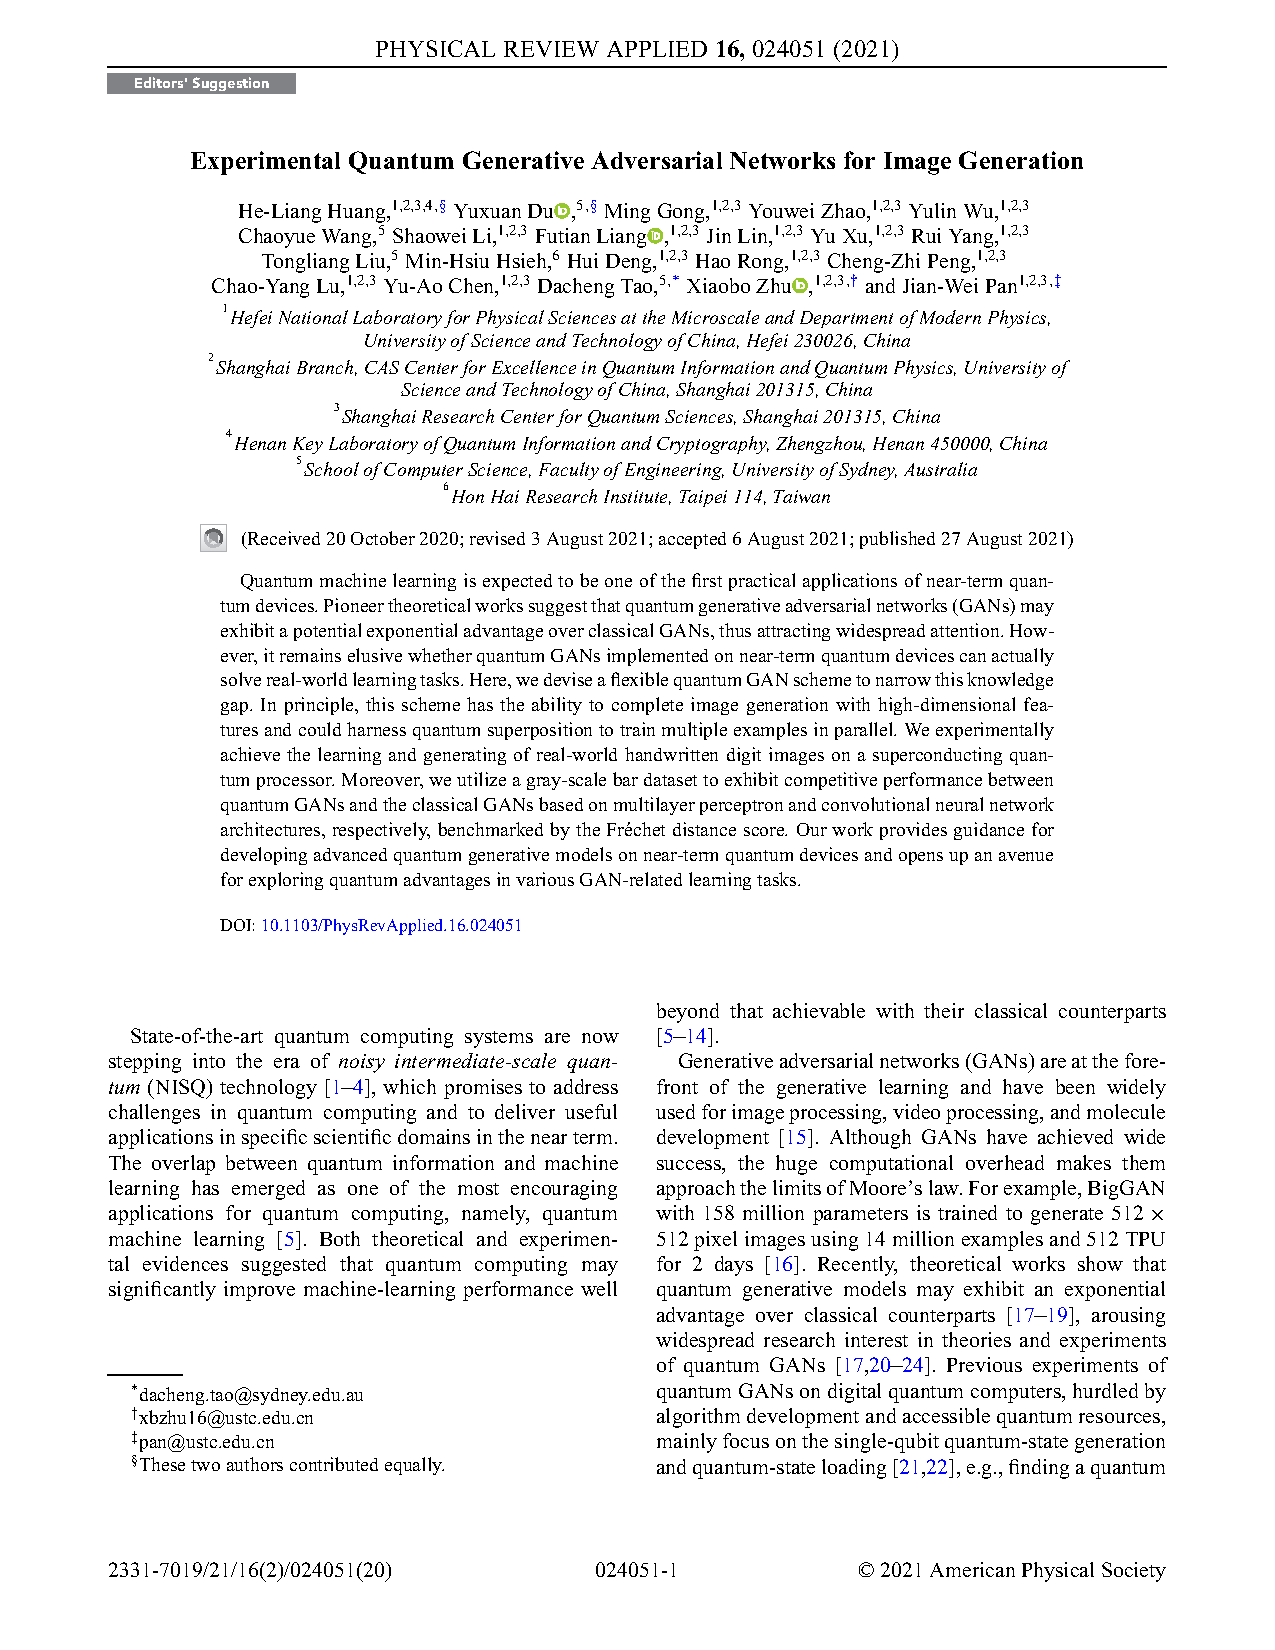
\includegraphics[width=0.8\linewidth,clip,frame,trim=0 500 0 0]{figures/paper-preview.pdf}%
    \\[-4em]%
    \begin{tikzpicture}
      \fill[white,path fading=north] (0,-3em) rectangle (0.81\linewidth,0);
      \fill[white] (0,-3em) rectangle (0.81\linewidth,-4em);
    \end{tikzpicture}% lol
  \end{center}
\end{frame}

\section{Mathematical preliminaries}

\begin{frame}
  \frametitle{Density matrices recap}

  In a pure state $\ket\psi$, the expected value of an observable $A$ is:

  \[ \expected{A}_\psi = \braopket{\psi}{A}{\psi} \]

  The probability of measuring the system in some basis can be found by using an
  orthogonal projector:

  \[ \Pi_i = \proj{\phi_i} \]

  In a mixed state $\rho$, the expected value looks like:

  \[ \expected{A}_\psi = \Tr(A \rho) = \sum_i \braopket{i}{A \rho}{i} \]

  (Trace is independent of basis---can sum over any basis $\{\ket{i}\}$)

\end{frame}

\begin{frame}
  \frametitle{Partial trace}

  If a measurement traces over a complete set of basis states for the space
  $\mathcal{H}$, what if we want to discard the subsystem $\mathcal{A}$ of
  $\mathcal{H}_{\mathcal{A}} \otimes \mathcal{H}_{\mathcal{B}}$?

  \[ \Tr_{\mathcal{A}}(\rho) =
  \sum_i (\bra{i}_{\mathcal{A}} \otimes I_{\mathcal{B}})
  \ \rho\ (\ket{i}_{\mathcal{A}} \otimes I_{\mathcal{B}})\]

  By \emph{tracing out} the system $\mathcal{A}$, we project onto a basis for
  $\mathcal{A}$ while leaving $\mathcal{B}$ untouched ($I_{\mathcal{B}}$).

  Each term of the sum leaves us with an \emph{operator} instead of a scalar.
  This is the \textbf{partial trace}\autocite{quic06}.

\end{frame}

\begin{frame}
  \frametitle{Partial trace example}

  \begin{center}
    \begin{quantikz}
      \lstick{$(\mathcal{A}) \ket{0}$} & \gate{H} & \ctrl{1} & \qw \\
      \lstick{$(\mathcal{B}) \ket{0}$} & \qw & \targ{} & \meter{}
    \end{quantikz}
  \end{center}

  We have prepared an entangled state:

  \[ \rho = \proj{\phi^+} = \frac{1}{2} \left( \proj{00} + \proj{11} \right) \]

  Let's trace out the first qubit.

  \[ \Tr_{\mathcal{A}}(\rho) = ? \]

\end{frame}

\begin{frame}
  \frametitle{Partial trace example}

  \begin{align*}
    \Tr_{\mathcal{A}}(\rho) &= \sum_i (\bra{i}_{\mathcal{A}} \otimes I_{\mathcal{B}}) \rho (\ket{i}_{\mathcal{A}} \otimes I_{\mathcal{B}}) \\
    \onslide<2->{
      &= \frac{1}{2} \sum_i \bigl( (\braket{i}{0} \braket{0}{i}) \otimes (I \proj{0} I) + (\braket{i}{1} \braket{1}{i}) \otimes (I \proj{1} I)\bigr) \\
    }
    \onslide<3->{
      &= \frac{1}{2} \bigl( 1 \otimes \proj{0} + 1 \otimes \proj{1} \bigr) \\
    }
    \onslide<4->{
      &= \frac{1}{2} \proj{+}
    }
  \end{align*}

  \onslide<4->{This is what we expected---ignoring the first qubit leaves our
    second qubit in the superposition $\ket{+}$.}

\end{frame}

\begin{frame}
  \frametitle{Partial measurement}

  What if we measure $\mathcal{A}$?  What we learn updates our density matrix
  for $\mathcal{B}$ (think conditional probabilities).

  Suppose we want to find the state of our system after measuring $\mathcal{A}$
  to be $\ket{i}$.

  \[\Pi_i \otimes I_{\mathcal{B}}\]

  Let's try the partial trace:

  \begin{align*}
    \Tr_{\mathcal{A}}((\Pi_i \otimes I_{\mathcal{B}}) \rho)
    &= \sum_j (\bra{j} \otimes I) (\Pi_i \otimes I) \rho (\ket{j} \otimes I) \\
    &= \sum_j (\bra{j} \Pi_i \otimes I) \rho (\ket{j} \otimes I) \\
  \end{align*}

\end{frame}

\begin{frame}
  \frametitle{Partial measurement}

  \[ \Tr_{\mathcal{A}}((\Pi_i \otimes I_{\mathcal{B}}) \rho) =
  \sum_j (\bra{j} \Pi_i \otimes I) \rho (\ket{j} \otimes I) \]

  Notice that $\bra{j} \Pi_j$ is $0$ if $i\neq j$, and $\bra{j}$ otherwise!

  \[ \Tr_{\mathcal{A}}((\Pi_i \otimes I_{\mathcal{B}}) \rho)
  = (\bra{i}\otimes I) \rho (\ket{i}\otimes I) \]

  We have picked out just the parts of $\rho$ that agree we our measurement, but
  the resulting operator may not be a density matrix (since the trace can be
  $<1$).

  \[ \rho' = \frac{\Tr_{\mathcal{A}}((\Pi_i\otimes I_{\mathcal{B}}) \rho)}
     {\Tr((\Pi_i\otimes I_{\mathcal{B}})\rho)} \]

\end{frame}

\begin{frame}
  \frametitle{Nonlinearity}

  Making a partial measurement on our system transforms the density matrix
  \emph{non-linearly}!

  \[ \rho' = \frac{\Tr_{\mathcal{A}}((\Pi_i\otimes I_{\mathcal{B}}) \rho)}
    {\LaTeXunderbrace{ \Tr((\Pi_i\otimes I_{\mathcal{B}})\rho) }_{\text{magic}}}\]

  The size of the ancillary system $\mathcal{A}$ influences ``how nonlinear''
  the outcome is.

\end{frame}

\begin{frame}[allowframebreaks]
  \frametitle{References}
  \printbibliography
\end{frame}

\end{document}
